% Options for packages loaded elsewhere
\PassOptionsToPackage{unicode}{hyperref}
\PassOptionsToPackage{hyphens}{url}
%
\documentclass[
  10pt,
]{article}
\usepackage{amsmath,amssymb}
\usepackage{iftex}
\ifPDFTeX
  \usepackage[T1]{fontenc}
  \usepackage[utf8]{inputenc}
  \usepackage{textcomp} % provide euro and other symbols
\else % if luatex or xetex
  \usepackage{unicode-math} % this also loads fontspec
  \defaultfontfeatures{Scale=MatchLowercase}
  \defaultfontfeatures[\rmfamily]{Ligatures=TeX,Scale=1}
\fi
\usepackage{lmodern}
\ifPDFTeX\else
  % xetex/luatex font selection
\fi
% Use upquote if available, for straight quotes in verbatim environments
\IfFileExists{upquote.sty}{\usepackage{upquote}}{}
\IfFileExists{microtype.sty}{% use microtype if available
  \usepackage[]{microtype}
  \UseMicrotypeSet[protrusion]{basicmath} % disable protrusion for tt fonts
}{}
\makeatletter
\@ifundefined{KOMAClassName}{% if non-KOMA class
  \IfFileExists{parskip.sty}{%
    \usepackage{parskip}
  }{% else
    \setlength{\parindent}{0pt}
    \setlength{\parskip}{6pt plus 2pt minus 1pt}}
}{% if KOMA class
  \KOMAoptions{parskip=half}}
\makeatother
\usepackage{xcolor}
\usepackage{longtable,booktabs,array}
\usepackage{calc} % for calculating minipage widths
% Correct order of tables after \paragraph or \subparagraph
\usepackage{etoolbox}
\makeatletter
\patchcmd\longtable{\par}{\if@noskipsec\mbox{}\fi\par}{}{}
\makeatother
% Allow footnotes in longtable head/foot
\IfFileExists{footnotehyper.sty}{\usepackage{footnotehyper}}{\usepackage{footnote}}
\makesavenoteenv{longtable}
\usepackage{graphicx}
\makeatletter
\def\maxwidth{\ifdim\Gin@nat@width>\linewidth\linewidth\else\Gin@nat@width\fi}
\def\maxheight{\ifdim\Gin@nat@height>\textheight\textheight\else\Gin@nat@height\fi}
\makeatother
% Scale images if necessary, so that they will not overflow the page
% margins by default, and it is still possible to overwrite the defaults
% using explicit options in \includegraphics[width, height, ...]{}
\setkeys{Gin}{width=\maxwidth,height=\maxheight,keepaspectratio}
% Set default figure placement to htbp
\makeatletter
\def\fps@figure{htbp}
\makeatother
\setlength{\emergencystretch}{3em} % prevent overfull lines
\providecommand{\tightlist}{%
  \setlength{\itemsep}{0pt}\setlength{\parskip}{0pt}}
\setcounter{secnumdepth}{-\maxdimen} % remove section numbering
% Official TMLR style; the preprint option avoids asserting an active review.
\usepackage[preprint]{tmlr}
\usepackage{microtype}
\fancyhead[L]{Research draft - not submitted}
\fancyhead[R]{1 October 2026}
\usepackage{fvextra}
\DefineVerbatimEnvironment{Highlighting}{Verbatim}{breaklines,commandchars=\\\{\}}
\AtBeginDocument{\maketitle\begin{abstract}Utility-constrained recommendations for DP-SGD depend on training
configuration, validation uncertainty and the environments used for
selection. We audit these decisions using matched ordinary,
clipping-only and noisy controls, frozen validation choices and held-out
ACS state tests. A synthetic study and ACS 2018 pilot motivate an
independently frozen ACS 2017 replication with 840 fits across two
representations. Joint configuration search produces successful
recommendations in all 20 seed cases per representation, compared with
zero or one for a restricted epsilon-only baseline. Source-only joint
search matches shift-aware search on this replication, so expansion of
the candidate bank explains the availability gain. A supplementary
400-fit comparison evaluates published AUTO-S clipping under a fixed
matched recipe. It produces no uncertainty-bound recommendations, while
standard norm search retains high yield; this is not a tuned algorithm
ranking. Fresh simultaneous calibration reproduces undercoverage in a
small rare-label clustered scenario (86.9\% against nominal 95\%). A
conservative concentration sensitivity covers every valid Gaussian
simulation but abstains on all ACS cases. These results support
configuration-sensitive decision auditing and explicit
coverage/abstention reporting, without a new mechanism, reliable ACS
certification or established general benefit of shift-aware selection.
\end{abstract}}
\ifLuaTeX
  \usepackage{selnolig}  % disable illegal ligatures
\fi
\IfFileExists{bookmark.sty}{\usepackage{bookmark}}{\usepackage{hyperref}}
\IfFileExists{xurl.sty}{\usepackage{xurl}}{} % add URL line breaks if available
\urlstyle{same}
\hypersetup{
  hidelinks,
  pdfcreator={LaTeX via pandoc}}

\title{Configuration and Uncertainty Sensitivity of DP-SGD Utility Recommendations: An ACS Decision Audit}
\author{Anonymous authors}
\date{}

\begin{document}
\maketitle

\hypertarget{research-question-and-relationship-to-the-msc}{%
\subsection{1. Research question and relationship to the
MSc}\label{research-question-and-relationship-to-the-msc}}

The original MSc compared privacy-related perturbations on a small
public insurance table, including smoker prediction with a strong
charges proxy. The revised benchmark introduced accounted DP-SGD,
leakage-safe evaluation and empirical privacy auditing. The present
study remains adjacent to that work through tabular prediction,
privacy-utility trade-offs and honest measurement, but asks a narrower
decision question:

\begin{quote}
When a validation rule recommends a DP-SGD budget subject to a relative
utility-loss margin and an absolute AUC floor, which recommendations
survive held-out distribution shift, and how sensitive is the answer to
clipping, training configuration and validation uncertainty?
\end{quote}

This study concerns utility reliability. It does not infer membership
privacy from utility, equate a failed attack with absence of leakage, or
revive the unsupported sex-specific leakage hypothesis. The earlier
LiRA/power work remains a separate study. Insurance motivates the
problem; controlled synthetic data and ACS provide the current evidence.

\hypertarget{closest-prior-work-and-bounded-contribution}{%
\subsection{2. Closest prior work and bounded
contribution}\label{closest-prior-work-and-bounded-contribution}}

Mahajan, Tople and Sharma {[}1{]} connect stable representations,
distribution generalization and membership inference, including utility
differences at the same formal DP guarantee. Therefore, discovering that
stable features can improve private utility is not a defensible novelty
claim here.

Zhang, Pang and Mauw {[}2{]} study privacy disparities associated with
spurious groups and the distinction between prediction robustness and
memorization. Our utility recommendation evaluation does not reproduce
their privacy conclusions or claim to introduce spurious-feature privacy
analysis.

DP-UTIL {[}3{]} compares utility and privacy across perturbation
locations. Bagdasaryan and Shmatikov {[}4{]} explain disparate accuracy
effects of clipping and noise. Consequently, broad mechanism comparisons
and the existence of clipping-related utility loss are established
background.

The candidate incremental contribution is a reproducible
\textbf{decision audit}: frozen validation-only budget choices; explicit
abstention and two failure criteria; matched clipping/noise controls;
paired clustered uncertainty; development separated from a prospective
synthetic primary comparison; and external state tests. None of these
ingredients alone is new. Their combination may support a useful
empirical benchmark, but a combination is not itself proof of
publication-level novelty. The results should be positioned as recipe
sensitivity and negative evidence against broad stress-test claims.

A subsequent targeted survey adds important constraints. Morsbach et
al.~{[}8{]} already establish joint clipping/learning-rate effects.
Panda et al.~{[}9{]} combine private HPO with OOD evaluation. DomainBed
{[}10{]} treats model selection as essential to domain generalization.
Accuracy First {[}11{]} and Brownian Noise Reduction {[}12{]} already
optimize privacy subject to accuracy requirements. Their methods analyze
the private release and adaptive utility checks; our fixed public-data
bank does not implement those mechanisms. Papernot and Steinke {[}16{]}
and Koskela and Kulkarni {[}17{]} likewise account for search privacy,
which is outside our per-candidate accounting. The supplementary
training comparator uses published AUTO-S {[}14{]}, not a new clipping
method. Consequently, neither the selection problem nor a joint search
is our method novelty. The
\href{../docs/CONFIGURATION_SELECTION_LITERATURE.md}{full survey} maps
sixteen related sources and the remaining evidence boundary.

\hypertarget{methods}{%
\subsection{3. Methods}\label{methods}}

\hypertarget{models-and-training-controls}{%
\subsubsection{3.1 Models and training
controls}\label{models-and-training-controls}}

The study uses a two-layer MLP (16 hidden units, tanh, one binary
logit), cross-entropy and SGD. All controls use matched initialization
and Poisson sampling streams with a common expected-batch gradient
normalization. The three conditions are ordinary training, per-record
clipped training with zero noise, and DP-SGD at requested
\(\varepsilon\) values 2 or 8. Noise uses a separate, fixed reproducible
random stream. The RDP accountant records achieved \(\varepsilon\),
\(\delta\)=\(10^{-5}\), sample rate, noise multiplier, steps and empty
batches per model.

Development uses 3,000 training rows, independent 2,000-row
validation/test cohorts, batch 256, 50 epochs and learning rate 0.1.
Synthetic development crosses strengths 0.75/0.90, clipping norms
0.5/1/2/5 and five seeds 10-14. ACS crosses norms 1/5 and the same five
seeds. These account for 160 and 40 model fits respectively, including
ordinary controls repeated across norms. Those repeated controls are not
independent observations.

This is a controlled recipe comparison, not a claim that each
configuration has been independently optimized. No alternative
architecture benchmark or convergence guarantee is established. Raising
the norm also raises absolute noise for a given noise multiplier, so the
contrast is a training-configuration effect rather than an isolated
causal effect of clipping.

\hypertarget{environments-and-data}{%
\subsubsection{3.2 Environments and data}\label{environments-and-data}}

The synthetic generator and all parameters are available in
\texttt{src/dp/proxy\_shift.py} and the JSON protocols. Train,
validation and test streams are independent within seed. Validation
proxy retention is 0.5/0.75; test retention is 0/0.25. Generic
perturbations provide a comparison validation rule. Proxy intervention
is controlled by construction, not inferred from real-world
correlations.

The external pilot downloads official 2018 one-year ACS person archives.
California supplies source train/validation/test partitions; Oregon and
Washington supply natural-shift validation; Nevada and Arizona supply
external tests. ACSIncome eligibility is age \textgreater16, income
\textgreater100, working hours \textgreater0 and person weight \(\geq\)
1, with binary target income \textgreater\$50,000 {[}5,6{]}.
Classification is unweighted and concerns public sampled records, not
survey-weighted population income estimates.

Encoding uses fixed public bounds for numeric features, fixed
categorical domains and deterministic modulo hashing for occupation and
birthplace. It differs from the standard Folktables representation.
Households are allocated wholly to distinct source partitions; the last
household in a partition can be truncated, with its unused records
excluded from subsequent partitions. Occupation-block zero masking is a
hypothetical validation stress test; it is not a causal explanation of
state differences. State shifts can change multiple variables and
relationships simultaneously.

ACS training seeds resample from the same fixed state archives, so they
are algorithm/cohort replications rather than independent state
replications. The five states and one year restrict external validity.

\hypertarget{recommendations-and-held-out-evaluation}{%
\subsubsection{3.3 Recommendations and held-out
evaluation}\label{recommendations-and-held-out-evaluation}}

For each configuration the recommendation chooses the smallest achieved
\(\varepsilon\) among candidate budgets satisfying both AUC loss
\(\leq\) 0.03 relative to the ordinary reference and private AUC
\(\geq\) 0.70 in every specified validation environment. Failure to meet
these constraints yields abstention. Source-only, proxy-stress and
generic/natural-shift rules are compared using point estimates or
uncertainty bounds. Privacy caps are fixed by the protocols, not
justified as acceptable deployment privacy levels.

All choices are persisted before external test scoring; ACS external
test records are loaded after choices are written. Test failure occurs
when either the relative gap exceeds 0.03 or private AUC falls below
0.70. Counts are reported alongside abstentions. Evaluations in two test
environments share a model and cannot be treated as independent
Bernoulli trials. Increasing abstention can reduce selected-case
failures without improving budget choice.

\hypertarget{paired-uncertainty-and-decomposition}{%
\subsubsection{3.4 Paired uncertainty and
decomposition}\label{paired-uncertainty-and-decomposition}}

AUC structural influences preserve ties and covariance between
predictions on the same labeled cohort. Variance sums record influences
within households for ACS, then uses a cluster sandwich estimate;
synthetic records form their own clusters. One-sided t bounds use a
Bonferroni family across validation environments, candidate budgets,
clipping norms and both gap/floor endpoints. At least 20 records per
class and 30 clusters are required. Boundary AUCs with degenerate
variance are marked unsupported rather than certified.

These are asymptotic, conditional-on-model bounds for sampled validation
environments. They do not certify unseen-state utility or constitute a
new confidence procedure. Cluster independence is an approximation for
ACS and does not model all survey design dependence. A Gaussian
clustered simulation and a paired household bootstrap provide limited
implementation/calibration checks; the broader simultaneous check in
Section 4.5 finds undercoverage in one small imbalanced scenario and
does not validate ACS survey-design coverage.

Let \(A^o\), \(A^c\), \(A^d\) denote ordinary, clipped and DP AUC. The
relative gap decomposes exactly as
(\(A^o\)-\(A^d\))=(\(A^o\)-\(A^c\))+(\(A^c\)-\(A^d\)). The corresponding
shift interaction subtracts the source gap from the shifted gap.
Components are matched training comparisons, not a general causal
mediation analysis; added-noise components can be negative.

\hypertarget{prospective-primary-comparison}{%
\subsubsection{3.5 Prospective primary
comparison}\label{prospective-primary-comparison}}

After development, the protocol fixed one primary contrast: norm-1 minus
norm-5 \textbf{total gap interaction}, at \(\varepsilon\)=2, strength
0.90 and test retention 0. The development paired SD was 0.0087875 AUC.
Normal-approximation planning used a 0.01 effect, two-sided
\(\alpha\)=0.05 and target power 0.80, with a minimum 20 fresh seeds.
The protocol uses seeds 100-119, 4,000 validation/test rows and
unchanged training settings. It was committed as \texttt{1feb9fe} before
that run started. This is a locally prospective protocol, not an
independently timestamped public preregistration. Five-seed variance
planning is uncertain.

The primary estimate uses the paired seed mean and Student-t 95\%
interval. All other confirmation-run summaries are descriptive. A
non-significant test does not imply equivalence; practical
interpretation must use the interval and the specified 0.01 margin. The
tested population is the specified synthetic generator/recipe, not
arbitrary tabular tasks.

\hypertarget{results}{%
\subsection{4. Results}\label{results}}

\hypertarget{synthetic-development}{%
\subsubsection{4.1 Synthetic development}\label{synthetic-development}}

At norm 0.5 and \(\varepsilon\)=2, mean complete-proxy-removal
interaction was approximately 0.02994 AUC, consisting of 0.02964
clipping-associated and 0.00030 added-noise components (pooled over both
development strengths for description only). At norm 1 the corresponding
mean was approximately 0.00093; at norm 5 it was approximately -0.00027.
These changes challenge a recipe-independent clipping-dominance story.
They also show why further mechanistic claims need stronger comparisons
than a single low-norm pilot.

Source-only selection failed in 12/20 held-out evaluations at norm 0.5
and 5/20 at norms 1, 2 and 5. Proxy stress at norm 0.5 selected seven of
ten seed/strength cases and failed in 6/14 evaluations; all higher-norm
rules selected ten cases and failed in 5/20. Point and bounded decisions
were equal in this development run. These counts do not demonstrate that
proxy stress generally improves transport. Absolute-floor violations can
remain when the ordinary reference also loses signal under shift.

\hypertarget{acs-external-pilot}{%
\subsubsection{4.2 ACS external pilot}\label{acs-external-pilot}}

At \(\varepsilon\)=2, ordinary/private source-test mean AUCs were
0.85578/0.82488 for norm 1 and 0.85578/0.84627 for norm 5. Norm-1 mean
clipped-only gradient clipping rate was approximately 54.9\%, versus
1.69\% for norm 5. Under norm 1, point source-only and natural-shift
rules each selected three seeds and failed in one of six external
evaluations; proxy stress selected two and failed in one of four.
Bounded selection abstained on all five seeds under every norm-1 rule.

Under norm 5, every rule and bound choice selected all five seeds and
all ten external evaluations passed. This is a pilot observation, not a
population failure-rate bound. Mean private AUC at \(\varepsilon\)=2 was
0.82875 in AZ and 0.81291 in NV; the corresponding ordinary means were
0.84276 and 0.82428. The larger norm reduces clipping-related source
utility loss here while leaving some added-noise loss. The external
relative gaps do not uniformly amplify source gaps; natural shift is not
equivalent to synthetic proxy removal.

\hypertarget{interval-checks}{%
\subsubsection{4.3 Interval checks}\label{interval-checks}}

Across 400 Gaussian clustered simulations, marginal one-sided 95\%
coverage was 0.950 for the gap upper bound and 0.960 for the AUC lower
bound. Nominal Monte Carlo standard error is 0.01090. This single DGP
does not validate ACS survey dependence, tail cases or simultaneous
selection coverage.

For the predetermined ACS source-validation seed-10, norm-1,
\(\varepsilon\)=2 cell, the paired influence gap upper bound was 0.03419
and the 999-replicate paired household percentile-bootstrap bound was
0.03436. Candidate AUC lower bounds were 0.82184 and 0.82052. Both
marginal gap bounds exceed the 0.03 tolerance. This is a sensitivity
check using two diagnostic retrains, not additional independent
experimental evidence or the multiplicity-adjusted selection rule.

\hypertarget{fresh-seed-primary-result}{%
\subsubsection{4.4 Fresh-seed primary
result}\label{fresh-seed-primary-result}}

The exact primary estimate and interval are recorded in the confirmation
stage's \texttt{primary\_result.json}. Across 20 fresh seeds, the norm-1
minus norm-5 interaction was \textbf{0.008275 AUC}, with paired-mean
95\% interval \textbf{{[}0.004092, 0.012458{]}} and two-sided
p=0.000556. The positive contrast is distinguishable from zero in the
specified experiment. Its interval straddles the planned 0.01
practical-effect margin; it establishes neither an effect above that
margin nor equivalence within that margin.

Descriptively, every rule selected all 20 seeds under both norms. Norm 1
failed in 20/40 held-out evaluations and norm 5 in 19/40; proxy stress
and bounded selection made the same choices as source-only selection.
These paired environment counts are not the primary statistical test and
do not establish a recommendation-policy improvement. There were 120
confirmation fits, including repeated ordinary controls.

\hypertarget{independent-acs-2017-configuration-selection-extension}{%
\subsubsection{4.5 Independent ACS 2017 configuration-selection
extension}\label{independent-acs-2017-configuration-selection-extension}}

Before external scoring, a separate protocol fixed CA source, OR/WA
validation and previously unused CO/UT external tests. Twenty fresh
seeds 200-219 were run for each of the original hashed representation
and a public decimal-digit one-hot sensitivity. Three recipes (16-unit
MLP/50 epochs/LR .1, 32-unit MLP/100 epochs/LR .05, logistic/100
epochs/LR .1), norms 1/5 and epsilon 2/8 provide 420 fits per encoding,
\textbf{840 in total}. Cohort sizes, batch size and utility limits
remain 3000/2000, 256, .03 gap and .70 floor. The common ordinary
reference is selected using source-validation AUC only. All decisions
and the reference are persisted before loading external tests. The
confidence family also covers every possible ordinary reference choice.

The primary endpoint is successful recommendation yield over all
seed/cohort cases; a selected case must satisfy both utility constraints
in both external states. Abstention is zero successful yield. At zero
safety margin, bounded fixed-recipe epsilon/source selection succeeds in
0/20 hashed and 1/20 digit cases, versus 20/20 for joint-recipe/shift
search. \textbf{Source-only joint clipping and source-only joint recipe
search also succeed in 20/20 under both encodings.} The primary yield
contrast is therefore +1.00 and +.95, but demonstrates no additional
success-yield benefit from shift-aware validation over competent
source-only configuration search. Search sizes differ; this is not a
claim of HPO efficiency or new selection methodology.

The original specified paired t summary is retained, with its degenerate
hashed interval flagged unsupported. A dated supplementary conservative
paired binary construction uses Bonferroni-combined Clopper-Pearson
discordance intervals: {[}.6065,1.0000{]} and {[}.5239,.9994{]}. These
intervals concern independent seed streams on a fixed split, not
independent states or universal transport. The supplementary estimator
is standard and does not fix AUC-bound coverage.

The point fixed-recipe source policy succeeds in 10/20 hashed cases (ten
abstentions), and 17/20 digit cases (one abstention, two selected
failures). Representation changes recommendation behavior. Bounded
logistic-only shift selection also succeeds in all 20 cases under each
encoding. Both source-only and shift-aware joint policies continue to
succeed in 20/20 at safety margin .01. All predefined margin curves and
exact-coverage comparisons are retained; no threshold is optimized
against test failures.

For the hashed base MLP at epsilon 2, mean source clipping/noise gaps
are .02884/.00136 at norm 1, versus .00010/.01153 at norm 5. This
illustrates a bias/noise balance under the same accounted privacy
target. The stronger MLP has similar ordinary utility, and does not
eliminate configuration sensitivity. These descriptive components are
not a general causal mechanism claim.

The full-family diagnostic has 600 clustered Gaussian simulations with
12 candidates, five environments and three possible references (360
endpoints). Observed simultaneous coverage is .880/.945/.980 in three
predefined imbalance/cluster scenarios; Monte Carlo SEs are
.0230/.0161/.0099. The .880 result limits any claim of uniform nominal
.95 calibration. The \texttt{bounds\_supported} flag checks
computational nondegeneracy, not coverage. The study uses explicitly
asymptotic estimates and does not provide certified utility.
\href{../reports/configuration_selection/FINDINGS.md}{Detailed findings
and provenance} retain the complete protocols, launch hashes, archive
checksums and accounting.

\hypertarget{supplementary-published-clipping-comparison}{%
\subsubsection{4.6 Supplementary published-clipping
comparison}\label{supplementary-published-clipping-comparison}}

After inspecting the original replication and calibration outcomes, we
froze a dated supplementary protocol and used new seeds 300-319 on the
same known ACS 2017 split. This is supplementary evidence, not a new
independent-domain confirmation. Each representation adds 200 fits: one
ordinary reference, three transformed/noise-free controls and six DP
candidates per seed. AUTO-S {[}14{]} uses all-parameter per-example
normalization \(g_i/(\lVert g_i\rVert_2+.01)\), unit sensitivity and the
same Opacus noise, expected-batch normalization and accounting. Standard
C=1/C=5 and AUTO-S share the base 16-unit MLP, 50 epochs and LR .1.
These fixed choices are not tuned after test outcomes and do not
reproduce the published vision/NLP suite.

All rules have the same 36-endpoint validation family and fixed ordinary
reference. This differs from Section 4.5's 360-endpoint bank/reference
family; cross-study yield changes do not isolate an algorithm effect.
Within this supplement, successful cases require both CO and UT to meet
the original gap .03 and AUC floor .70. The following rows use safety
margin zero:

\begin{longtable}[]{@{}llrr@{}}
\toprule\noalign{}
Representation & Selection / uncertainty & Selected & Successful \\
\midrule\noalign{}
\endhead
\bottomrule\noalign{}
\endlastfoot
Hashed & AUTO-S source / point & 0/20 & 0/20 \\
Hashed & AUTO-S source / sandwich & 0/20 & 0/20 \\
Hashed & Standard joint source / point or sandwich & 20/20 & 20/20 \\
Hashed & Combined shift / point or sandwich & 20/20 & 20/20 \\
Digits & AUTO-S source / point & 10/20 & 5/20 \\
Digits & AUTO-S shift / point & 2/20 & 2/20 \\
Digits & AUTO-S source or shift / sandwich & 0/20 & 0/20 \\
Digits & Standard joint source / point or sandwich & 20/20 & 19/20 \\
Digits & Combined shift / point or sandwich & 20/20 & 20/20 \\
Both & Every policy / concentration sensitivity & 0/20 & 0/20 \\
\end{longtable}

AUTO-S does not improve recommendation yield under this one schedule.
This does not establish inferiority after appropriate
learning-rate/epoch tuning. Combined shift versus combined source has
yield difference 0 for hashing and .05 for digits. Conservative paired
seed-case intervals are {[}-.1968,.1968{]} and {[}-.1961,.2793{]},
respectively. The digit gain is one case; the interval includes zero and
does not establish a reliable shift-validation benefit. These are
supplementary descriptive contrasts, not multiplicity-adjusted
confirmatory tests. Both standard source and shift joint rules had 20/20
success in the original independent replication; retain both findings.

\begin{figure}
\centering
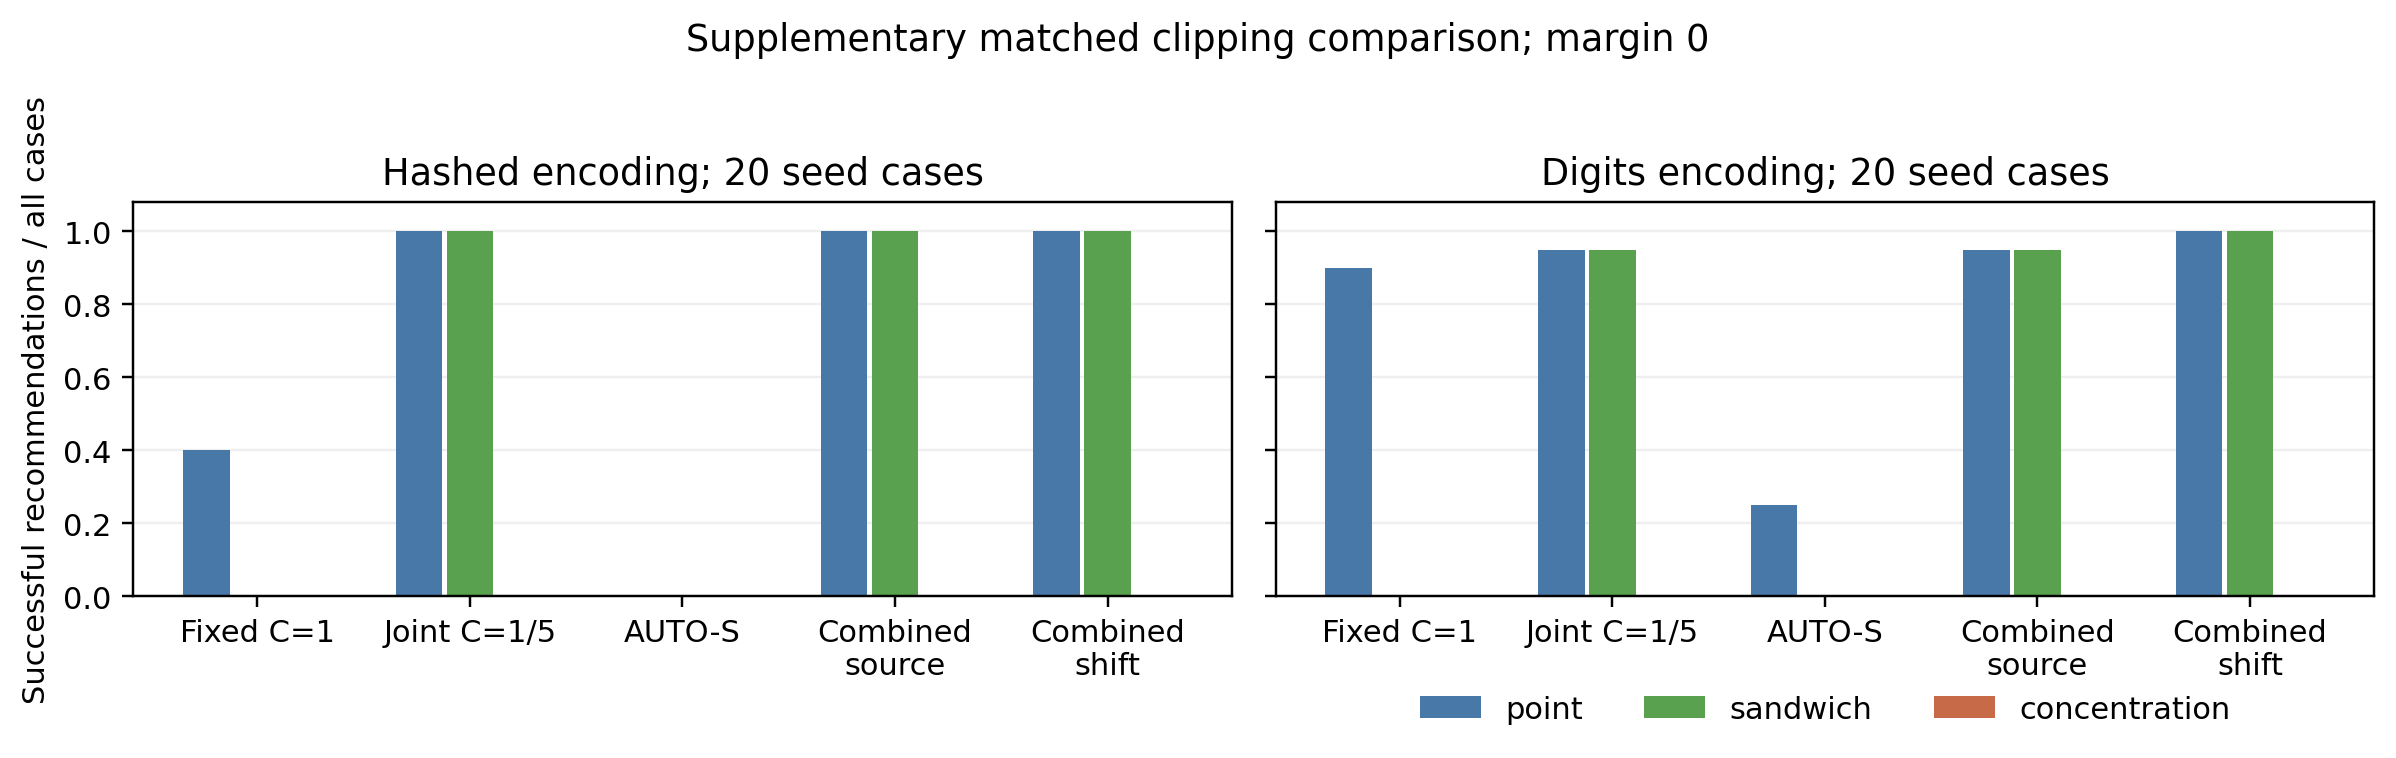
\includegraphics{../../reports/configuration_selection/clipping_comparison.png}
\caption{Successful recommendation yield for the supplementary matched
clipping study. The conservative sensitivity abstains for every policy.}
\end{figure}

\hypertarget{fresh-calibration-and-a-conservative-sensitivity}{%
\subsubsection{4.7 Fresh calibration and a conservative
sensitivity}\label{fresh-calibration-and-a-conservative-sensitivity}}

Fresh simulation seed 20261002 repeats the three known Gaussian
clustered scenarios with 200 draws each and the original 360 endpoints.
One rare-label draw has fewer than 20 records/class and is excluded by
the original validity rule; 599 draws are valid. The original sandwich
procedure is unchanged.

\begin{longtable}[]{@{}
  >{\raggedright\arraybackslash}p{(\columnwidth - 8\tabcolsep) * \real{0.1765}}
  >{\raggedleft\arraybackslash}p{(\columnwidth - 8\tabcolsep) * \real{0.2353}}
  >{\raggedright\arraybackslash}p{(\columnwidth - 8\tabcolsep) * \real{0.1765}}
  >{\raggedleft\arraybackslash}p{(\columnwidth - 8\tabcolsep) * \real{0.2353}}
  >{\raggedright\arraybackslash}p{(\columnwidth - 8\tabcolsep) * \real{0.1765}}@{}}
\toprule\noalign{}
\begin{minipage}[b]{\linewidth}\raggedright
Prevalence / households
\end{minipage} & \begin{minipage}[b]{\linewidth}\raggedleft
Sandwich simultaneous coverage
\end{minipage} & \begin{minipage}[b]{\linewidth}\raggedright
Exact binomial 95\% interval
\end{minipage} & \begin{minipage}[b]{\linewidth}\raggedleft
Concentration coverage
\end{minipage} & \begin{minipage}[b]{\linewidth}\raggedright
Mean raw gap radius: sandwich / concentration
\end{minipage} \\
\midrule\noalign{}
\endhead
\bottomrule\noalign{}
\endlastfoot
.10 / 100 & 173/199 (.8693) & {[}.8144,.9128{]} & 199/199 & .1404 /
1.1472 \\
.30 / 250 & 191/200 (.9550) & {[}.9163,.9792{]} & 200/200 & .0653 /
.5901 \\
.50 / 250 & 194/200 (.9700) & {[}.9358,.9889{]} & 200/200 & .0486 /
.5704 \\
\end{longtable}

The rare-label failure reproduces the original .880 coverage result. It
cannot be repaired by relabelling a nondegenerate computation as
supported inference. The manuscript therefore retains sandwich selection
as an asymptotic heuristic and removes dependable certification from its
contribution claim.

For a conservative sensitivity, apply standard bounded differences
{[}15{]} to independent score-generating households conditional on the
label vector and cluster membership. With P/N positive/negative records
and household counts \(p_h,n_h\), changing a household's scores affects
at most \(c_h=p_h/P+n_h/N-p_hn_h/(PN)\) of all positive-negative rank
pairs. Let \(r=\sqrt{\tfrac12\sum_h c_h^2\log(M/\alpha)}\) and
\(w=\sum_h p_hn_h/(PN)\), where M is the endpoint family. A
candidate-AUC kernel has range {[}0,1{]}; a paired-gap kernel has range
{[}-1,1{]}. Conditional-expectation radii are r and 2r. Under a common
class-conditional marginal score law across households \textbf{after
conditioning on the entire label vector}, within-household pair bias
relative to the marginal target is bounded by w and 2w. Use candidate
lower AUC \(\widehat A-r-w\) and upper gap \(\widehat G+2r+2w\).

These conditions hold in the simulated score DGP, but need not hold in
ACS: households may be dependent and conditional score laws may vary
with their labels and other attributes. Thus concentration selection on
ACS is an assumption-dependent sensitivity, not a survey-design or
unseen-state certificate. All 599 valid simulations are covered; the
coverage lower confidence limits are about .982, not proof of universal
coverage. The bounds are so wide that every ACS rule abstains, even at
zero safety margin. Exact seed-yield intervals do not remedy AUC
uncertainty or survey assumptions.

\begin{figure}
\centering
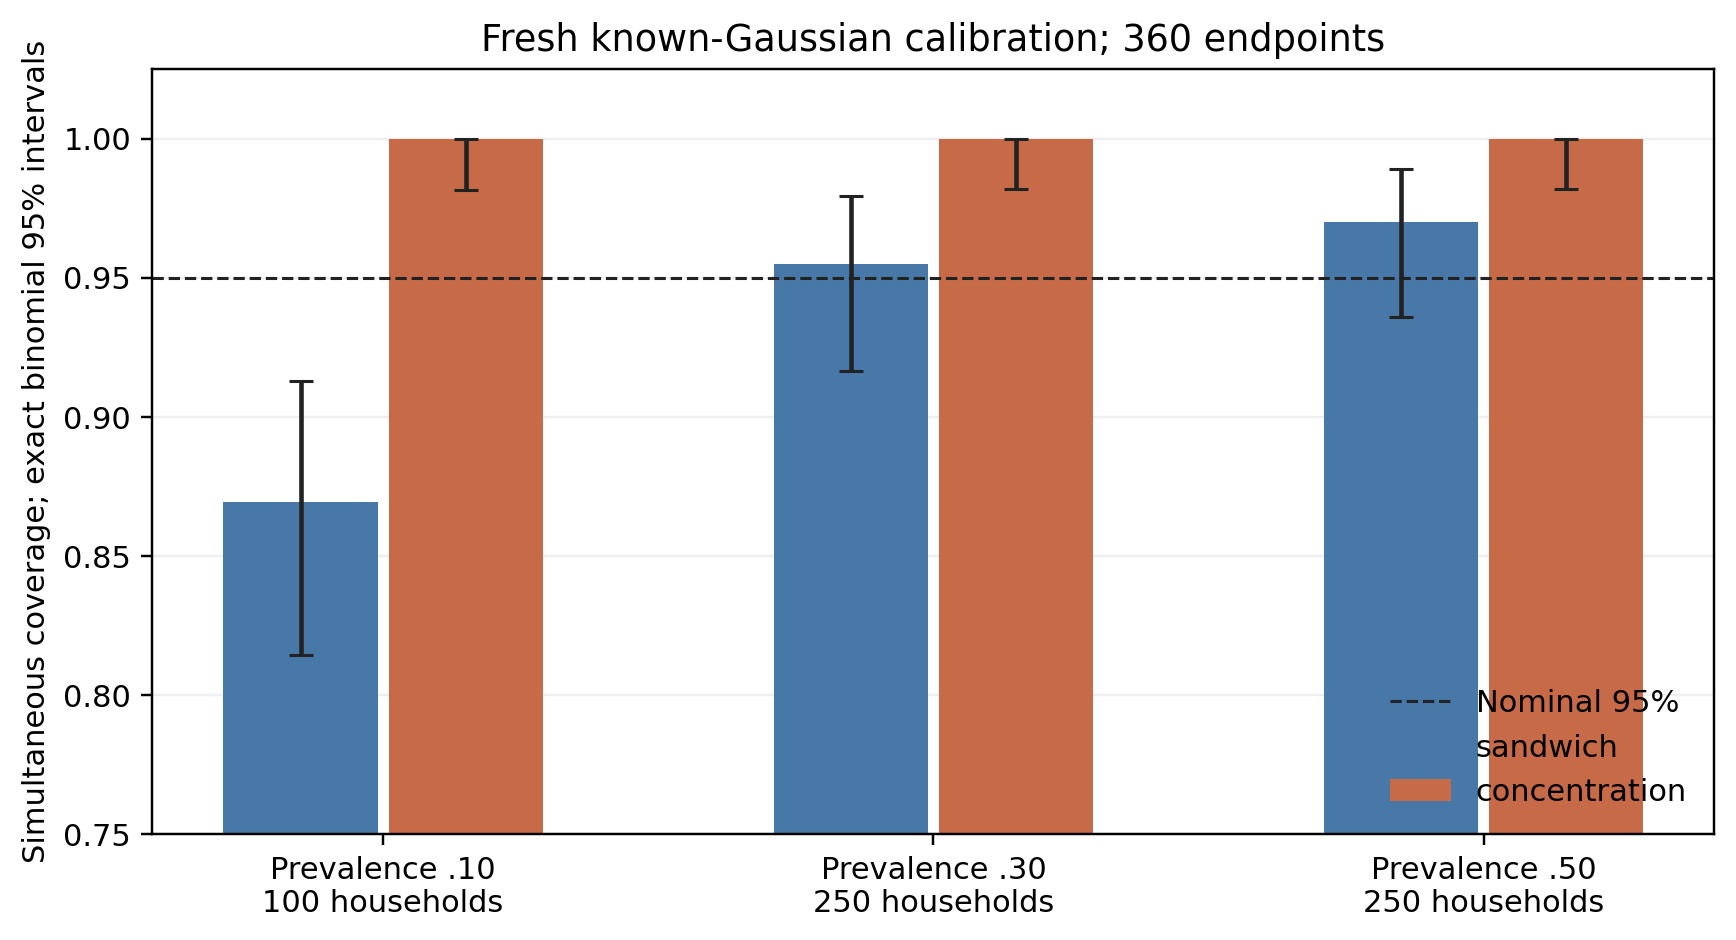
\includegraphics{../../reports/configuration_selection/calibration_followup.png}
\caption{Fresh complete-family calibration. Error bars describe Monte
Carlo coverage uncertainty; they are not ACS validation intervals.}
\end{figure}

\hypertarget{interpretation-and-submission-boundary}{%
\subsection{5. Interpretation and submission
boundary}\label{interpretation-and-submission-boundary}}

The evidence currently supports checking clipping/training configuration
before telling a privacy-noise or proxy-robustness story, and reporting
abstention alongside selected-case failures. It does not establish a new
DP protection phenomenon or universally superior recommendation policy.
Related work already establishes the broad stable-feature and
clipping/noise issues. The defensible publication direction is a narrow
reproducible benchmark/negative-result contribution, subject to a
reviewer finding the decision evaluation increment useful.

The independently frozen ACS replication, representation sensitivity and
stronger recipe/logistic comparison have now been executed (Section
4.5). They narrow the interpretation to configuration-sensitive
recommendation availability; shift-aware search adds no successful-yield
improvement on the examined splits. Before submission, assess scholarly
novelty and venue fit against the expanded full-text/citation-chain
review. The supplementary AUTO-S comparison and fresh calibration
response now run (Sections 4.6-4.7). Reliable operational certification
is excluded: the sandwich rule undercovers and the assumption-dependent
conservative fallback abstains. A useful, well-calibrated operational
selector remains future work. Appropriate tuning and a faithfully
implemented private-HPO comparator would be required for
algorithm/search superiority, which is not claimed here. ACS is already
implemented and executed, so another unrelated dataset is optional for
this narrow claim. It becomes necessary if claiming cross-domain
generality. The tiny insurance table cannot provide that generality
merely by remaining in the paper. A stronger non-neural baseline,
selected only on validation data, would help establish that failures are
not an undertrained MLP artifact; the original extension already
includes a validation-selected logistic comparison. No automated script
can guarantee sufficient scholarly novelty. TMLR's replication-friendly
criteria provide a plausible route to assess reader interest, without
establishing acceptance. Author and external expert review remain
necessary before an actual submission.

\hypertarget{privacy-scope-reproducibility-and-limitations}{%
\subsection{6. Privacy scope, reproducibility and
limitations}\label{privacy-scope-reproducibility-and-limitations}}

The Opacus accountant covers each prepared-record DP-SGD model under the
implemented Poisson sampling and add/remove adjacency. It does not
account for the many-model research release, public evaluation/selection
or the older insurance preprocessing. Fixed public ACS encoding avoids
learning feature domains from private records, but household-safe
partitions and household-cluster utility inference do not provide
household DP. The study uses public data and reproducible
non-cryptographic randomness; it is not a production privacy deployment
or an acceptable-\(\varepsilon\) policy.

Configs, per-model accounting, frozen choices, metrics, decisions,
archive checksums and calibration results are committed. Raw ACS
archives and prepared records are excluded from Git. Runtime/provenance
notes identify executed revisions, including the development runner's
stage-label metadata change during execution. Reported source hashes
captured at run completion must not be mistaken for an immutable launch
snapshot.

Commands and the prospective protocol are in
\texttt{docs/PUBLICATION\_PLAN.md}. Reproduction requires a fresh output
directory, the listed CPU runtime and official data access. Seeds
reproduce experimental streams conditional on software/hardware; tests
check invariants rather than certify scientific conclusions. The
historical PDF and unsupported demographic significance claims must not
be used as the submission manuscript.

The supplementary protocol was committed locally before launch; its
identical tree was pushed during execution. Source hashes verify no
training-code change between launch and completed manifests. It is not
independently registered, and the external state/year outcomes were
already known. A source-equivalent public protocol snapshot is commit
\texttt{9fe78890ed716b2f4ec808d7f3389d326acc203a}. The new
run-verification checks account for all 400 fits, frozen choices and
their subsequent decisions. They validate saved invariants, not a second
full reproduction or the statistical assumptions.

\hypertarget{references}{%
\subsection{References}\label{references}}

\begin{enumerate}
\def\labelenumi{\arabic{enumi}.}
\tightlist
\item
  Mahajan, D., Tople, S., Sharma, A. (2021). \emph{The Connection
  between Out-of-Distribution Generalization and Privacy of ML Models}.
  \url{https://arxiv.org/abs/2110.03369}
\item
  Zhang, C., Pang, J., Mauw, S. (2025). \emph{Spurious Privacy Leakage
  in Neural Networks}. TMLR. https://arxiv.org/abs/2505.20095
\item
  Jarin, I., Eshete, B. (2022). \emph{DP-UTIL: Comprehensive Utility
  Analysis of Differential Privacy in Machine Learning}. CODASPY.
  \url{https://arxiv.org/abs/2112.12998}
\item
  Bagdasaryan, E., Shmatikov, V. (2019). \emph{Differential Privacy Has
  Disparate Impact on Model Accuracy}. https://arxiv.org/abs/1905.12101
\item
  Ding, F., Hardt, M., Miller, J., Schmidt, L. (2021). \emph{Retiring
  Adult: New Datasets for Fair Machine Learning}.
  \url{https://github.com/socialfoundations/folktables}
\item
  U.S. Census Bureau. 2018 ACS one-year PUMS person archives.
  \url{https://www2.census.gov/programs-surveys/acs/data/pums/2018/1-Year/}
\item
  Ying, G., Maguire, M. G., Glynn, R. J., Rosner, B. (2022; online
  2021). \emph{Tutorial on Biostatistics: Receiver-Operating
  Characteristic (ROC) Analysis for Correlated Eye Data}. Ophthalmic
  Epidemiology, 29(2), 117-127.
  \url{https://pmc.ncbi.nlm.nih.gov/articles/PMC8586066/}
\item
  Morsbach, F., Reubold, J., Strufe, T. (2024). \emph{R+R: Understanding
  Hyperparameter Effects in DP-SGD}. ACSAC.
  https://arxiv.org/abs/2411.02051
\item
  Panda, A., Tang, X., Mahloujifar, S., Sehwag, V., Mittal, P. (2024).
  \emph{A New Linear Scaling Rule for Private Adaptive Hyperparameter
  Optimization}. ICML. https://proceedings.mlr.press/v235/panda24a.html
\item
  Gulrajani, I., Lopez-Paz, D. (2021). \emph{In Search of Lost Domain
  Generalization}. ICLR. https://arxiv.org/abs/2007.01434
\item
  Ligett, K., Neel, S., Roth, A., Waggoner, B., Wu, Z. S. (2017).
  \emph{Accuracy First: Selecting a Differential Privacy Level for
  Accuracy-Constrained ERM}. NeurIPS. https://arxiv.org/abs/1705.10829
\item
  Whitehouse, J., Wu, Z. S., Ramdas, A., Rogers, R. (2022).
  \emph{Brownian Noise Reduction: Maximizing Privacy Subject to Accuracy
  Constraints}. NeurIPS. https://arxiv.org/abs/2206.07234
\item
  U.S. Census Bureau. 2017 ACS one-year PUMS person archives.
  \url{https://www2.census.gov/programs-surveys/acs/data/pums/2017/1-Year/}
\item
  Bu, Z., Wang, Y.-X., Zha, S., Karypis, G. (2023). \emph{Automatic
  Clipping: Differentially Private Deep Learning Made Easier and
  Stronger}. NeurIPS.
  \url{https://proceedings.neurips.cc/paper_files/paper/2023/hash/8249b30d877c91611fd8c7aa6ac2b5fe-Abstract-Conference.html}
\item
  Warnke, L. (2016; online 2015). \emph{On the Method of Typical Bounded
  Differences}. Combinatorics, Probability and Computing, 25(2),
  269-299. Standard bounded differences is background here; the present
  study does not use its typical-differences extension.
  \url{https://arxiv.org/abs/1212.5796}
\item
  Papernot, N., Steinke, T. (2022). \emph{Hyperparameter Tuning with
  Renyi Differential Privacy}. ICLR. https://arxiv.org/abs/2110.03620
\item
  Koskela, A., Kulkarni, T. (2023). \emph{Practical Differentially
  Private Hyperparameter Tuning with Subsampling}. NeurIPS.
  \url{https://papers.neurips.cc/paper_files/paper/2023/file/59b9582cd35f555ea8415030073e7b22-Paper-Conference.pdf}
\end{enumerate}

\end{document}
